\subsection{Canal soma ruído}
% harvard HW5_ES250_sol.pdf - q1
\begin{questions}
\question{
Encontre a capacidade de canal do seguinte canal discreto sem memória:
\begin{figure}[h!]
\centering
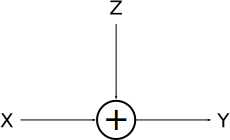
\includegraphics[width=0.2\linewidth]{../images/xplusz.pdf}
\label{fig:q2}
\end{figure}
onde $Pr\{Z=0\} = Pr\{Z=a\} = \frac{1}{2}$. Temos que o alfabeto de $x$ é
$\mathcal{X} = \{0,1\}$ e o alfabeto de $z$ é $\mathcal{Z} = \{0,a\}$. 
Assuma que $Z$ seja independente de $X$. Observe que a capacidade
de canal depende do valor $a$.


}


\begin{solution}
\begin{eqnarray}
C &=& \max_{p(x)} I(X;Y) \nonumber \\
        &=& \max_{p(x)} H(Y) - H(Y|X) \nonumber \\
        &=& \max_{p(x)} H(Y) - H(Z)
\end{eqnarray}
onde utilizamos que
\begin{equation}
H(Y|X) = H(Z|X) = H(Z) = \begin{cases} 1 , \quad a \neq 0 \\ 0, \quad a = 0 \end{cases}.
\end{equation}

Podemos também utilizar
\begin{eqnarray}
C &=& \max_{p(x)} I(X;Y) \\
        &=& \max_{p(x)} H(X) - H(X|Y) 
\end{eqnarray}

Será necessário agora determinar o alfabeto de $Y$. 
Note que $\mathcal{Y}$ dependerá do valor de $a$.

\begin{enumerate}
\item[para $a = 0$]: neste caso, $\mathcal{Y} = \{0,1\}$. Neste caso, $Y=X$ e, por conseguinte,
$H(Y) = H(X)$. Sabemos que $H(X) \leq 1$, logo teremos $C=1$ bits por utilização do canal. 
\item[para $a = 1$]: neste caso, $\mathcal{Y} = \{0,1,2\}$. O canal se comporta como um
canal binário com apagamento.

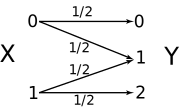
\includegraphics[width=0.3\textwidth]{../images/canalapagamento.pdf}

Como visto em aula, a capacidade deste canal será $C = 1 - \alpha$, onde $\alpha = 1/2$,
logo $C = 1/2$ bit por transmissão.

\item[para $a = -1$]: neste caso, $\mathcal{Y} = \{-1,0,1\}$. Caso similar ao caso em que $a=1$. 
Teremos novamente $C = 1/2$ bit por transmissão.

\item[para $a \neq 0, \pm 1$]: neste caso, $\mathcal{Y} = \{0,1,a,1+a\}$. Neste caso, conhecendo $Y$
sabemos quem foi o $X$ enviado, assim $H(X|Y) = 0$.
\begin{eqnarray}
C &=& \max_{p(x)} I(X;Y) \nonumber \\
        &=& \max_{p(x)} H(X) - \underbrace{H(X|Y)}_{=0} = \max_{p(x)} H(X) = 1
\end{eqnarray}
A capacidade será atingida quando $X \sim \text{uniforme}$. 
\end{enumerate}



\end{solution}
\end{questions}
